\documentclass[tikz,border=8pt]{standalone}
\usepackage{amsmath,amssymb}
\usetikzlibrary{arrows.meta,calc,decorations.markings,decorations.pathmorphing,patterns,shapes.geometric,positioning}

\begin{document}
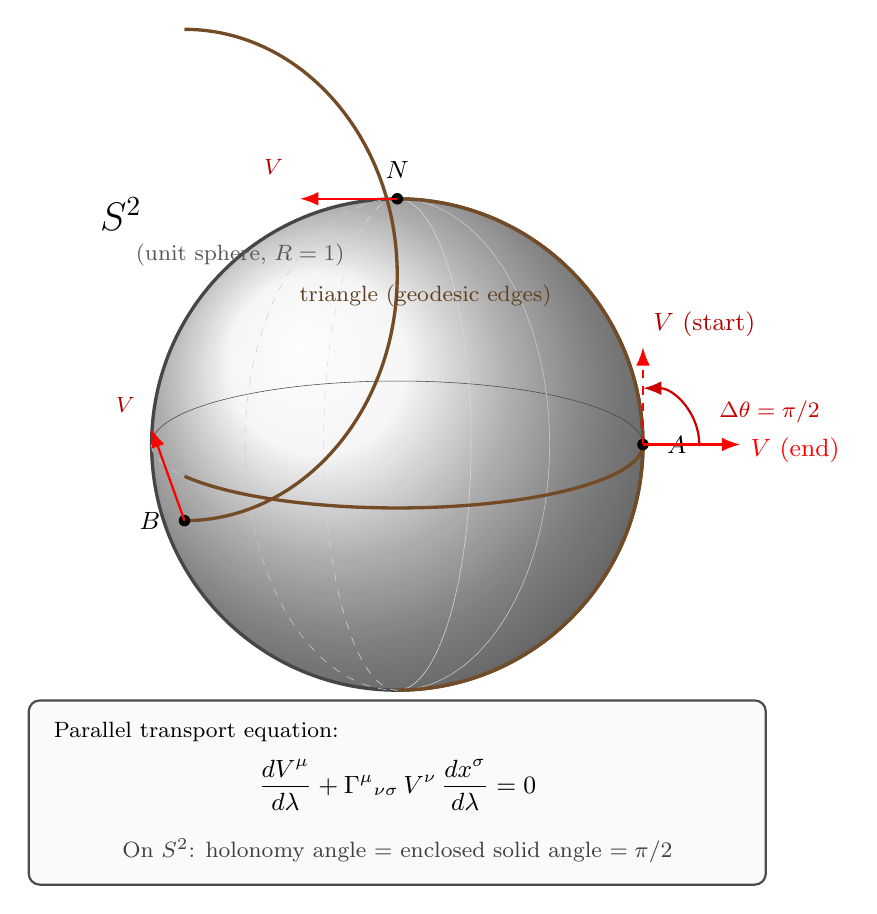
\begin{tikzpicture}[>=Latex, scale=1.30]

  % =====================================================================
  % Sphere S^2 with a triangular loop A -> B -> N -> A and parallel
  % transport of a vector V; final vector at A is rotated by pi/2.
  % =====================================================================

  \def\R{2.4}              % sphere radius (drawing units)
  \def\Yflat{0.62}          % vertical squash for ellipses (perspective)

  % ---- 1. Sphere body, shaded ----
  \shade[ball color=gray!10, opacity=0.95] (0,0) circle (\R);
  \draw[very thick, gray!55!black] (0,0) circle (\R);

  % ---- 2. Equator (front solid, back dashed) ----
  \draw[gray!50, dashed, thin]
        (-\R, 0) arc (180:360:{\R} and \Yflat);
  \draw[gray!55!black, very thin]
        ( \R, 0) arc (0:180:{\R} and \Yflat);

  % a couple of meridian guide lines (very faint)
  \draw[gray!40, dashed, very thin]
        (0,\R) arc (90:270:{0.62*\R} and \R);
  \draw[gray!40, very thin]
        (0,\R) arc (90:-90:{0.62*\R} and \R);
  \draw[gray!30, dashed, very thin]
        (0,\R) arc (90:270:{0.30*\R} and \R);
  \draw[gray!30, very thin]
        (0,\R) arc (90:-90:{0.30*\R} and \R);

  % ---- 3. Three triangle vertices ----
  % A : equator, phi = 0  (front-right of sphere)
  % B : equator, phi = pi/2 (front-left in drawing, we put it left-front)
  % N : north pole (top)
  \coordinate (Apt)  at ({\R}, 0);
  \coordinate (Bpt)  at ({-0.10*\R}, {0.18*\Yflat});  % near front, but we use a clean position below
  \coordinate (Npt)  at (0, {\R});

  % put B more clearly: phi=90 deg on the equator front
  % using parametric form: x = R cos(phi), y = Yflat * R sin(phi) but we want it visible
  % Choose B at phi = 110 deg (gives a slightly back-left nice spot)
  \coordinate (Bpt)  at ({\R*cos(110)}, {\Yflat*\R*sin(110)*0 + (-0.05)});
  % Actually we want B on equator front at phi=90, drawn at x=0, y=0:
  \coordinate (Bpt)  at (0, 0);

  % Better: use phi=120 deg so B is on the front-left arc of equator
  \coordinate (Bpt)  at ({\R*cos(135)}, {-\Yflat*\R*sin(135)*0.0});
  % Force B to lie on visible front arc of equator with proper y dip
  \coordinate (Bpt)  at ({\R*cos(150)}, {-\Yflat*\R*sin(150)});

  % ---- 4. Triangle edges (dark brown) ----
  % Edge A -> B : equator arc on front (from phi=0 toward phi increasing to ~150 deg, taking the front lower part)
  % Front equator arc from A (0 deg) going clockwise through y<0 to B at 150 deg of equator
  \draw[very thick, brown!60!black]
        (\R, 0) arc (0:-150:{\R} and \Yflat);

  % Edge B -> N : meridian from B up to north pole
  % B is at (R cos150, -Yflat R sin150). The meridian semi-axis (half-width) = |x_B| = R |cos150|
  \pgfmathsetmacro{\hwB}{\R*0.866}     % |cos 150| = 0.866
  \draw[very thick, brown!60!black]
        (Bpt) arc (-90:90:{\hwB} and \R);

  % Edge N -> A : meridian from N down to A
  % A is at (R, 0). Its meridian half-width = R.
  \draw[very thick, brown!60!black]
        (0, \R) arc (90:-90:{\R} and \R);

  % Mark vertices
  \fill[black] (Apt) circle (1.6pt);
  \fill[black] (Bpt) circle (1.6pt);
  \fill[black] (Npt) circle (1.6pt);

  \node[font=\small, anchor=west] at ([xshift=4pt]Apt) {$A$};
  \node[font=\small, anchor=east] at ([xshift=-4pt]Bpt) {$B$};
  \node[font=\small, anchor=south] at ([yshift=3pt]Npt) {$N$};

  % ---- 5. Initial vector V at A : pointing North along meridian (upward in plane) ----
  % dashed (reference / original direction)
  \draw[red, dashed, thick, ->]
        (Apt) -- ++(0, 0.95)
        node[anchor=south west, font=\small, red!70!black] {$V$ (start)};

  % ---- 6. Vector at B after first leg ----
  % After parallel transport along equator arc, V at B still points "north"
  % i.e. perpendicular to equator at B, which is along the meridian direction at B.
  % At B (phi=150), the local "north" tangent is in the direction
  %   (-sin(180-150) * |cos(...)|... ) -- to keep it intuitive we draw it tangent to the meridian going up.
  % The meridian-up direction at B is the unit tangent of the BN arc at B.
  % The arc center for the meridian B->N is at (0,0). At B the tangent to that arc going toward N
  % is perpendicular to (Bpt - origin), rotated 90 deg toward N.
  \pgfmathsetmacro{\bx}{\R*cos(150)}
  \pgfmathsetmacro{\by}{-\Yflat*\R*sin(150)}
  \pgfmathsetmacro{\rmag}{sqrt(\bx*\bx + \by*\by)}
  \pgfmathsetmacro{\nx}{-\by/\rmag}
  \pgfmathsetmacro{\ny}{\bx/\rmag}
  % We want it to point toward N (upward in y), so flip sign if ny<0
  \pgfmathsetmacro{\sgn}{ifthenelse(\ny>0, 1, -1)}
  \pgfmathsetmacro{\Vbx}{0.95*\sgn*\nx}
  \pgfmathsetmacro{\Vby}{0.95*\sgn*\ny}

  \draw[red, thick, ->]
        (Bpt) -- ++(\Vbx, \Vby);
  \node[font=\footnotesize, red!70!black, anchor=south east]
        at ([xshift=-2pt, yshift=2pt]$ (Bpt) + (\Vbx, \Vby) $) {$V$};

  % ---- 7. Vector at N after second leg ----
  % After transport along meridian B->N, V at N is rotated relative to the next meridian
  % so that it lies along the BN meridian's "tangent at N" pointing back toward B side.
  % At N, draw V pointing in the direction of B's meridian (toward B).
  % That direction is opposite to the unit vector from N to A along its meridian.
  % A's meridian direction at N: tangent of arc N->A at N points toward A, i.e. (1, 0) direction (down-east in y, but actually horizontal at the pole).
  % B's meridian direction at N: tangent of arc B->N at N points back toward B, which is in direction (cos150, ...) ~ (-0.87, 0).
  % So V at N points roughly (-1, 0).
  \draw[red, thick, ->]
        (Npt) -- ++(-0.95, 0);
  \node[font=\footnotesize, red!70!black, anchor=south east]
        at ([xshift=-2pt, yshift=4pt]$ (Npt) + (-0.95, 0) $) {$V$};

  % ---- 8. Final vector at A after third leg ----
  % After transport from N down meridian to A, V is now perpendicular to original (which was "north"="up").
  % It is rotated by pi/2 -- we draw it horizontal pointing south of east, i.e. tangent to the equator.
  % Specifically: original V at A was (0, +1); final V at A is rotated by pi/2 clockwise (from the viewer side):
  % (0,1) -> (1, 0), i.e. eastward along the equator.
  \draw[red, thick, ->]
        (Apt) -- ++(0.95, 0)
        node[anchor=west, font=\small, red, yshift=-2pt]
            {$V$ (end)};

  % ---- 9. Rotation angle arc at A ----
  \draw[->, thick, red!80!black]
        ([xshift=0.55cm]Apt) arc (0:90:0.55cm);
  \node[font=\footnotesize, red!80!black, anchor=west]
        at ([xshift=0.65cm, yshift=0.32cm]Apt) {$\Delta\theta=\pi/2$};

  % ---- 10. Sphere label ----
  \node[font=\Large\bfseries] at (-2.7, 2.25) {$S^2$};
  \node[font=\footnotesize, gray!70!black, anchor=west] at (-2.65, 1.85) {(unit sphere, $R=1$)};

  % ---- 11. Bottom formula box: parallel transport ODE ----
  \begin{scope}[shift={(0, -3.4)}]
    \draw[rounded corners=4pt, thick, gray!60!black, fill=gray!4]
          (-3.6, -0.9) rectangle (3.6, 0.9);
    \node[font=\footnotesize, anchor=north west] at (-3.45, 0.78)
        {Parallel transport equation:};
    \node[font=\small, anchor=north] at (0, 0.42)
        {$\dfrac{dV^{\mu}}{d\lambda}
          + \Gamma^{\mu}{}_{\nu\sigma}\, V^{\nu}\,
            \dfrac{dx^{\sigma}}{d\lambda} = 0$};
    \node[font=\footnotesize, gray!50!black, anchor=south]
          at (0, -0.78)
          {On $S^{2}$: holonomy angle $=$ enclosed solid angle $= \pi/2$};
  \end{scope}

  % ---- 12. Triangle area annotation ----
  \node[font=\footnotesize, brown!50!black, anchor=west]
        at (-1.05, 1.45) {triangle (geodesic edges)};

\end{tikzpicture}
\end{document}
